\section{Big data}

Controlling the full potential of big data requires a well-structured data management process that spans every stage of the data pipeline. 
The essential components of this process include:
\begin{enumerate}
    \item \textit{Data collection}: the foundation of any big data initiative lies in gathering information from diverse sources. 
    \item \textit{Data analysis}: the data must be carefully analyzed to extract meaningful patterns, trends, and insights. 
        This step often involves tailoring the analysis to meet the needs of specific stakeholders. 
        Techniques include:
        \begin{itemize}
            \item Descriptive analysis: providing a clear picture of current trends and performance.
            \item Predictive analysis: using historical data to forecast future scenarios and behaviors.
        \end{itemize}
    \item \textit{Value creation}: the ultimate goal of the data pipeline is to transform raw data into actionable insights that drive value for organizations, enabling informed decision-making and innovation.
\end{enumerate} 
\noindent Big data's growing prominence is driven by several critical factors:
\begin{itemize}
    \item \textit{Decreasing storage costs}: advances in storage technology have significantly reduced costs, allowing organizations to store massive datasets affordably.
        This affordability makes it practical to collect and analyze large volumes of data on a regular basis.
    \item \textit{Ubiquitous data generation}: in our digital age, data is generated everywhere. 
    \item \textit{Rapid data growth}: the volume of data is increasing at a pace far greater than IT budgets. 
        This mismatch underscores the urgency for scalable and efficient data management solutions to handle the ever-growing data demands across industries.
\end{itemize}
\begin{table}[h!]
    \centering
    \begin{tabular}{|l|p{10cm}|}
    \hline
    \textbf{Dimension} & \textbf{Description} \\ \hline
    \textit{Volume}    & Refers to the immense scale of data generated and stored. Big data encompasses vast quantities, ranging from terabytes to exabytes, made possible by increasingly affordable storage solutions \\ \hline
    \textit{Variety}   & Describes the diverse forms in which data is available. Big data includes structured data, unstructured data, and multimedia content \\ \hline
    \textit{Velocity}  & Represents the speed at which data is generated, processed, and analyzed. Big data often involves real-time or near-real-time data streams, enabling rapid decision-making within fractions of a second \\ \hline
    \textit{Veracity}  & Concerns the uncertainty and reliability of data. Big data often includes information that may be imprecise, incomplete, or uncertain, requiring robust methods to manage and ensure data accuracy and predictability \\ \hline
    \end{tabular}
    \caption{The four V's of Big Data}
\end{table}
    
\subsection{Data analysis}
As the volume of data continues to grow, our methods for addressing data-related challenges must adapt accordingly. 
Traditional approaches to data analysis were constrained by processing limitations, often relying on small subsets of data. 
In contrast, big data enables a paradigm shift, allowing for the analysis of entire datasets, leading to more comprehensive understanding and deeper insights.
\begin{figure}[H]
    \centering
    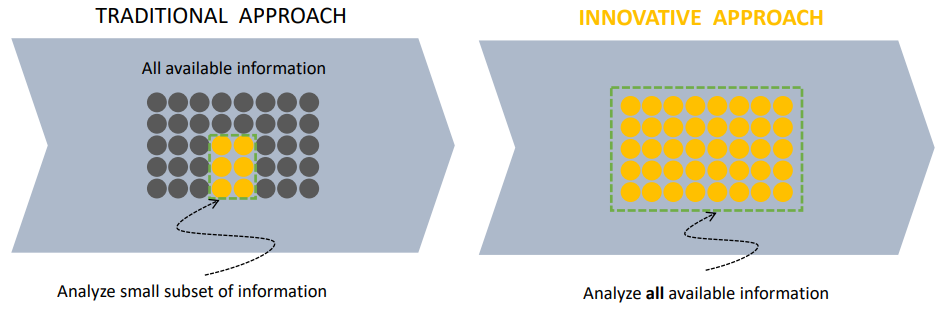
\includegraphics[width=0.75\linewidth]{images/in.png}
    \caption{Data analysis}
\end{figure}
\noindent In traditional analysis, a hypothesis is formed and tested against a small, pre-selected dataset.
While useful, this method limits discoveries to the scope of the sample.
In the big data approach, all available data is explored, uncovering correlations and patterns without requiring predefined hypotheses. 
This data-driven exploration reveals insights that traditional methods might overlook.
\begin{figure}[H]
    \centering
    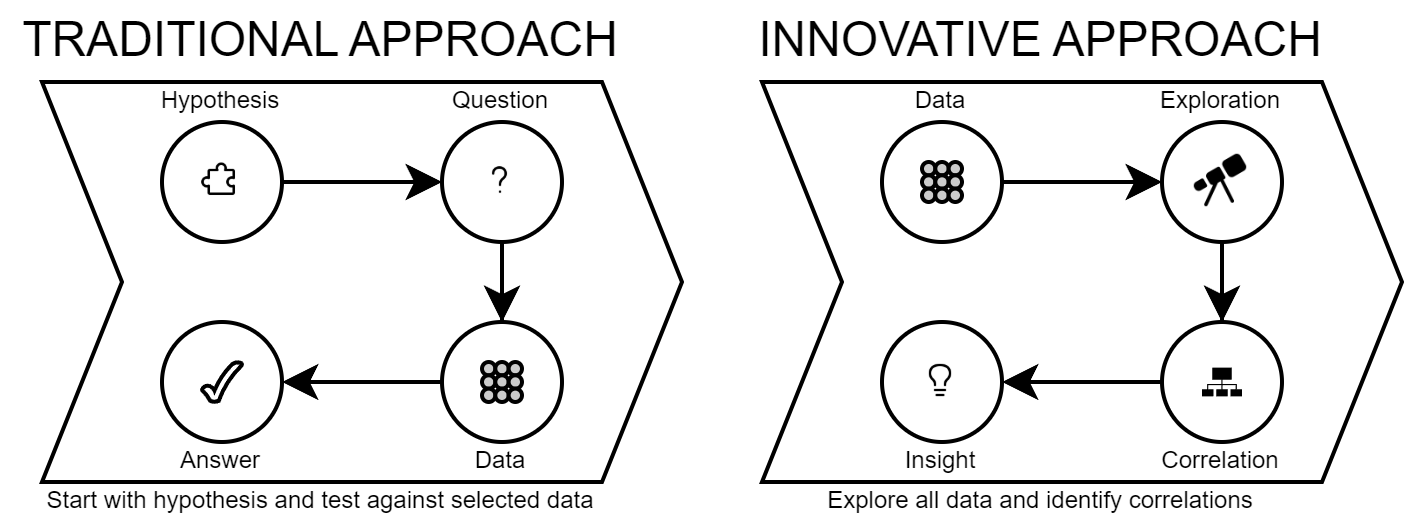
\includegraphics[width=0.75\linewidth]{images/in1.png}
    \caption{Data-driven analysis}
\end{figure}
\noindent Traditional methods require extensive data cleansing before analysis, resulting in a smaller but highly organized dataset.
Big data, on the other hand, embraces the messiness of raw data, analyzing it first and cleansing as necessary. 
This approach enables the processing of larger volumes of less structured data.
\begin{figure}[H]
    \centering
    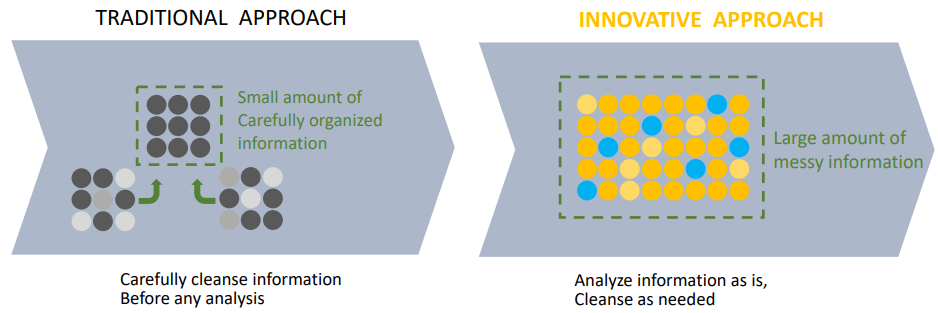
\includegraphics[width=0.75\linewidth]{images/in2.png}
    \caption{Data cleaning}
\end{figure}
\noindent Traditional techniques often involve analyzing data only after it has been processed and stored in a data warehouse or mart.
Big data leverages real-time analysis, processing data as it is generated. 
This enables timely insights and faster decision-making.
\begin{figure}[H]
    \centering
    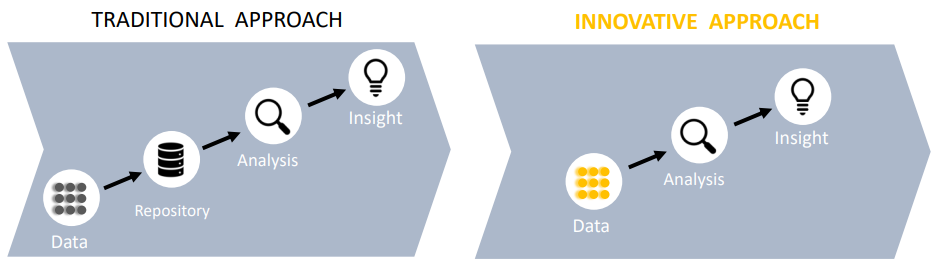
\includegraphics[width=0.75\linewidth]{images/in3.png}
    \caption{Real-time analysis}
\end{figure}